\section{Resultados}\label{sec:resultados}

\subsection{Primer experimento: Comprobaci�n de que los tres rayos
involucrados y la normal est�n en el mismo plano}\label{subsec:primero}

\usetikzlibrary{arrows,shapes,positioning}
\usetikzlibrary{decorations.markings}
\tikzstyle arrowstyle=[scale=1]
\tikzstyle directed=[postaction={decorate,decoration={markings,
mark=at position .65 with {\arrow[arrowstyle]{stealth}}}}]
\tikzstyle reverse directed=[postaction={decorate,decoration={markings,
mark=at position .65 with {\arrowreversed[arrowstyle]{stealth};}}}]

\begin{figure}[tbh]
    \begin{center}
        \begin{tikzpicture}

            % define coordinates
            \coordinate (O) at (0,0);
            \coordinate (A) at (0,4);
            \coordinate (B) at (0,-3);
            \coordinate (TL) at (-4,4);
            \coordinate (TR) at (4,4);
            \coordinate (BL) at (-4,-3);
            \coordinate (BR) at (4,-3);

            \draw[thick] (-3,0) -- (3,0) arc(0:180:3) --cycle;
            \begin{scope}
                \clip (-3,0) rectangle (3,3);
                \fill[blue!60!,opacity=.3] (0,0) circle(3);
            \end{scope}

            % media
            \fill[blue!25!,opacity=.3] (TL) rectangle (BR);

            \node[right] at (1,0.5) {Vidrio};
            \node[left] at (-2.5,2.5) {Aire};

            % axis
            \draw[dash pattern=on5pt off3pt] (A) -- (B);

            % rays
            \draw[red,ultra thick,reverse directed] (O) -- (130:-3.9);
            \draw[blue,directed,ultra thick] (O) -- (-70:-4.24);
            \draw[green,directed,ultra thick] (O) -- (-130:3.9);

            % angles
            \draw (0,1) arc (90:110:1);
            \draw (0,-1) arc (270:310:1);
            \draw (0,-1) arc (270:230:1);
            \node[] at (290:1.4)  {$\theta_{i}$};
            \node[] at (250:1.4)  {$\theta_{r}$};
            \node[] at (100:1.4)  {$\theta_{t}$};
        \end{tikzpicture}
        \caption{Configuraci�n 1 del dispositivo.}
        \label{fig:dispositivo1}
    \end{center}
\end{figure}


\begin{figure}[tbh]
    \begin{center}
        \begin{tikzpicture}

            % define coordinates
            \coordinate (O) at (0,0);
            \coordinate (A) at (0,4);
            \coordinate (B) at (0,-2);
            \coordinate (TL) at (-4,4);
            \coordinate (TR) at (4,4);
            \coordinate (BL) at (-4,-2);
            \coordinate (BR) at (4,-2);

            \draw[thick] (-3,0) -- (3,0) arc(0:180:3) --cycle;
            \begin{scope}
                \clip (-3,0) rectangle (3,3);
                \fill[blue!60!,opacity=.3] (0,0) circle(3);
            \end{scope}

            % media
            \fill[blue!25!,opacity=.3] (TL) rectangle (BR);

            \node[right] at (1,0.5) {Vidrio};
            \node[left] at (-2.5,2.5) {Aire};

            % axis
            \draw[dash pattern=on5pt off3pt] (A) -- (B);

            % rays
            \draw[red,ultra thick,reverse directed] (O) -- (-130:-5.2);
            \draw[blue,directed,ultra thick] (O) -- (20:-4.24);
            \draw[green,directed,ultra thick] (O) -- (130:5.2);

            % angles
            \draw (0,1) arc (90:50:1);
            \draw (0,1) arc (90:130:1);
            \draw (0,-1) arc (270:200:1);
            \node[] at (70:1.4)  {$\theta_{i}$};
            \node[] at (235:1.4)  {$\theta_{t}$};
            \node[] at (110:1.4)  {$\theta_{r}$};
        \end{tikzpicture}
        \caption{Configuraci�n 2 del dispositivo.}
        \label{fig:dispositivo2}
    \end{center}
\end{figure}

\subsection{Segundo experimento: Medida de los �ngulos de reflexi�n y refracci�n}\label{subsec:segundo}

\begin{table}[h!]
    \center
    \caption{�ngulos de incidencia $\theta_i$, de reflexi�n $\theta_r$ y de refracci�n $\theta_t$.}
    \label{tab:radio}
    \begin{centering}
        \begin{tabular}{|P{40px}|P{40px}|P{40px}|}
            \hline
            $\theta_i\,$(\textdegree) & $\theta_r\,$(\textdegree) & $\theta_t\,$(\textdegree)              \\
            \hline
            \csvreader[late after line= \\, /csv/separator=semicolon ]{./files/data/segundo_es.csv}{}% use head of csv as column names
            {\csvcoli                 & \csvcolii                 & \csvcoliii    }% specify your columns here
            \hline
        \end{tabular}
    \end{centering}
\end{table}

\subsubsection{Comprobaci�n de la ley de la reflexi�n}

\begin{figure}[tbh]
    \begin{center}
        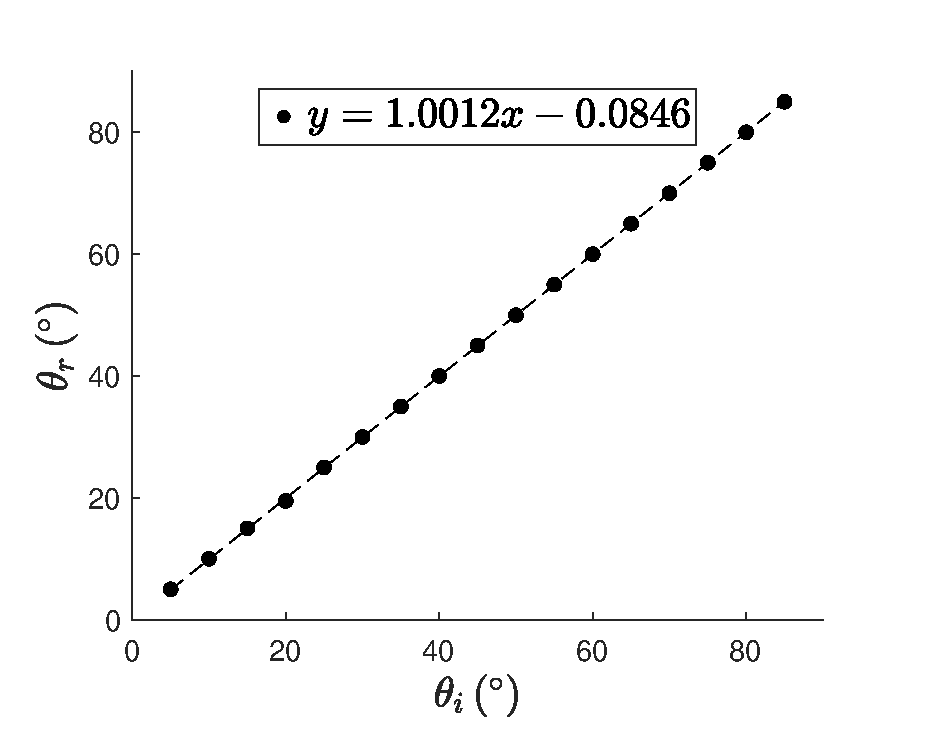
\includegraphics[width=0.8\columnwidth]{files/images/reflexion}
    \end{center}
    \caption{�ngulo de reflexi�n $\theta_r$ frente al �ngulo de incidencia $\theta_i$.}
    \label{fig:reflexion}
\end{figure}

\FloatBarrier

\begin{equation*}
    m = 1.0012 \pm 0.0012
    \hspace{10px}; \hspace{10px}
    b = -0.08\text{\textdegree} \pm 0.06\text{\textdegree}
\end{equation*}

\FloatBarrier

\subsubsection{Comprobaci�n de la ley de Snell o de la refracci�n}

\begin{figure}[tbh]
    \begin{center}
        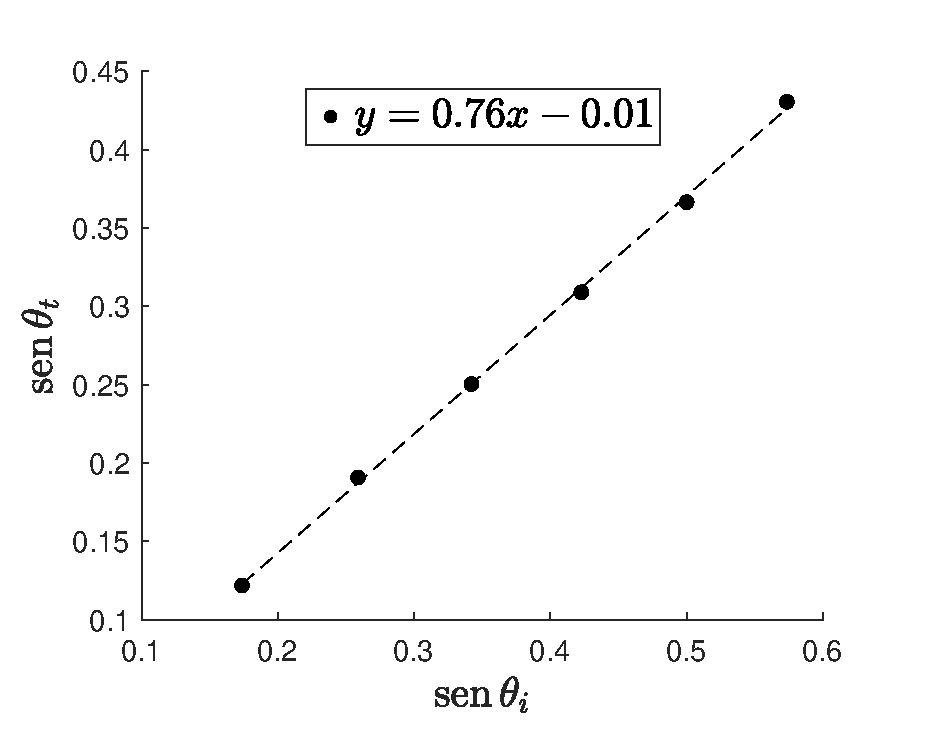
\includegraphics[width=0.8\columnwidth]{files/images/refraccion}
    \end{center}
    \caption{Seno del �ngulo de refracci�n $\theta_t$ frente al seno del �ngulo de incidencia $\theta_i$.}
    \label{fig:refraccion}
\end{figure}


\FloatBarrier

\begin{equation*}
    m = 0.676 \pm 0.004
    \hspace{10px}; \hspace{10px}
    b = -0.001 \pm 0.003
\end{equation*}

\FloatBarrier

\subsubsection{Aproximaci�n paraxial o de Gauss}


\begin{figure}[tbh]
    \begin{center}
        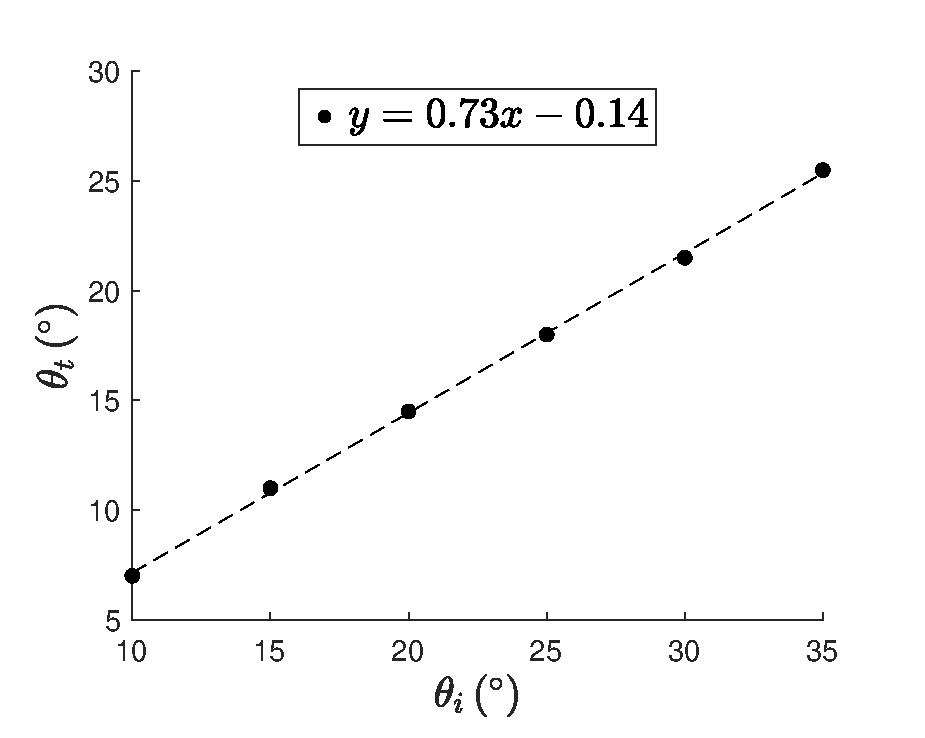
\includegraphics[width=0.8\columnwidth]{files/images/aproximacion}
    \end{center}
    \caption{�ngulo de refracci�n $\theta_t$ frente al �ngulo de incidencia $\theta_i$.}
    \label{fig:aproximacion}
\end{figure}

\FloatBarrier

\begin{equation*}
    m = 0.639 \pm 0.010
    \hspace{10px}; \hspace{10px}
    b = 0.4\text{\textdegree} \pm 0.2\text{\textdegree}
\end{equation*}

\FloatBarrier

\subsection{Tercer experimento: �ngulo l�mite}\label{subsec:tercero}


\begin{table}[h!]
    \center
    \caption{�ngulos de incidencia $\theta_i$ desde el agua en torno al �ngulo l�mite.}
    \label{tab:limite}
    \begin{centering}
        \begin{tabular}{|P{40px}|P{66px}|P{66px}|}
            \hline
            $\theta_i\,$(\textdegree) & Transmisi�n & No transmisi�n                         \\
            \hline
            \csvreader[late after line= \\, /csv/separator=semicolon ]{./files/data/limite.csv}{}% use head of csv as column names
            {\csvcoli                 & \csvcolii   & \csvcoliii    }% specify your columns here
            \hline
        \end{tabular}
    \end{centering}
\end{table}

Del an�lisis de la tabla~\ref{tab:limite} se deduce que el valor del �ngulo l�mite $\theta_t$ debe encontrarse entre
$42.0$\textdegree y $42.5$\textdegree.
Es decir, su valor se puede tomar como:
\begin{equation*}
    \theta_ t = 42.3\text{\textdegree} \pm 0.5\text{\textdegree}
\end{equation*}
